% =====================================
\section{Acoustic Features}
% =====================================
\subsection{Voice Quality Features}

The feature set used in this study, denoted as VQual, included $F_0$, $F_1$, $F_2$, $F_3$, harmonic amplitude differences $H_1$-$H_2$, $H_2$-$H_4$, $H_4$-$H_\mathrm{2k}$, formant amplitudes $A_1$, $A_2$, $A_3$, and cepstral peak prominence (CPP, [22]). Here, $H_1$, $H_2$, $H_4$, and $H_\mathrm{2k}$ indicate the amplitudes of first, second, fourth harmonics, and the harmonic nearest to 2 kHz, respectively. The first and second derivatives of these features were also used. Features were extracted using the VoiceSauce toolkit~\cite{shue2010voice}.

% An automatic estimation algorithm is available from the VoiceSauce toolkit [18]. 
% The first and second derivatives of these features were also used.
% %\Soo{I think we should include acoustic analysis. Like, the feature distribution plots for each sleepiness level. Because the performance improvement is not huge, this part will be more important than system description. However, the problem is that our data (e.g., decreasing F0, increasing speech rate) has opposite patterns from the acoustic characteristics of sleepiness in literature. We should have explanation for that.}

% In order to see if voice quality features are related to the degree of sleepiness, the mean value of voice quality features within each utterance was calculated, 
% and the mean and standard deviation were computed across the utterances of each degree of sleepiness.
% It was observed that the voice quality features varied according to the degree of sleepiness,
% and many of them had overall monotonically increasing or decreasing pattern along the KSS rating.

% For example, as shown in Figure~\ref{fig:vqual}, the mean $F_0$ values were positively correlated with the degree of sleepiness both for the training dataset ($\rho=0.81$, $p<0.05$) and the development dataset ($\rho=0.79$, $p<0.05$) between KSS ratings from 2 to 9. 
% Interestingly, this pattern was opposite from the literature that reported decreasing F0 with higher sleepiness. \Soo{This difference might be due to that ... } 

% \Soo{for H2-H4, H4-H2k} 

% Although the features were correlated for KSS ratings from 2 to 9, 
% the utterances of KSS rating 1 in the training dataset did not follow the pattern.
% It is difficult to make a conclusion based on this because the number of utterances were small for that case.
% A possible explanation can be that that specific case happened to include many more female speakers than male speakers, resulting in higher F0 values than other cases.
% This possibility could not be tested with the given dataset because no gender label was available.
 
% \begin{figure}
%     \centering
%     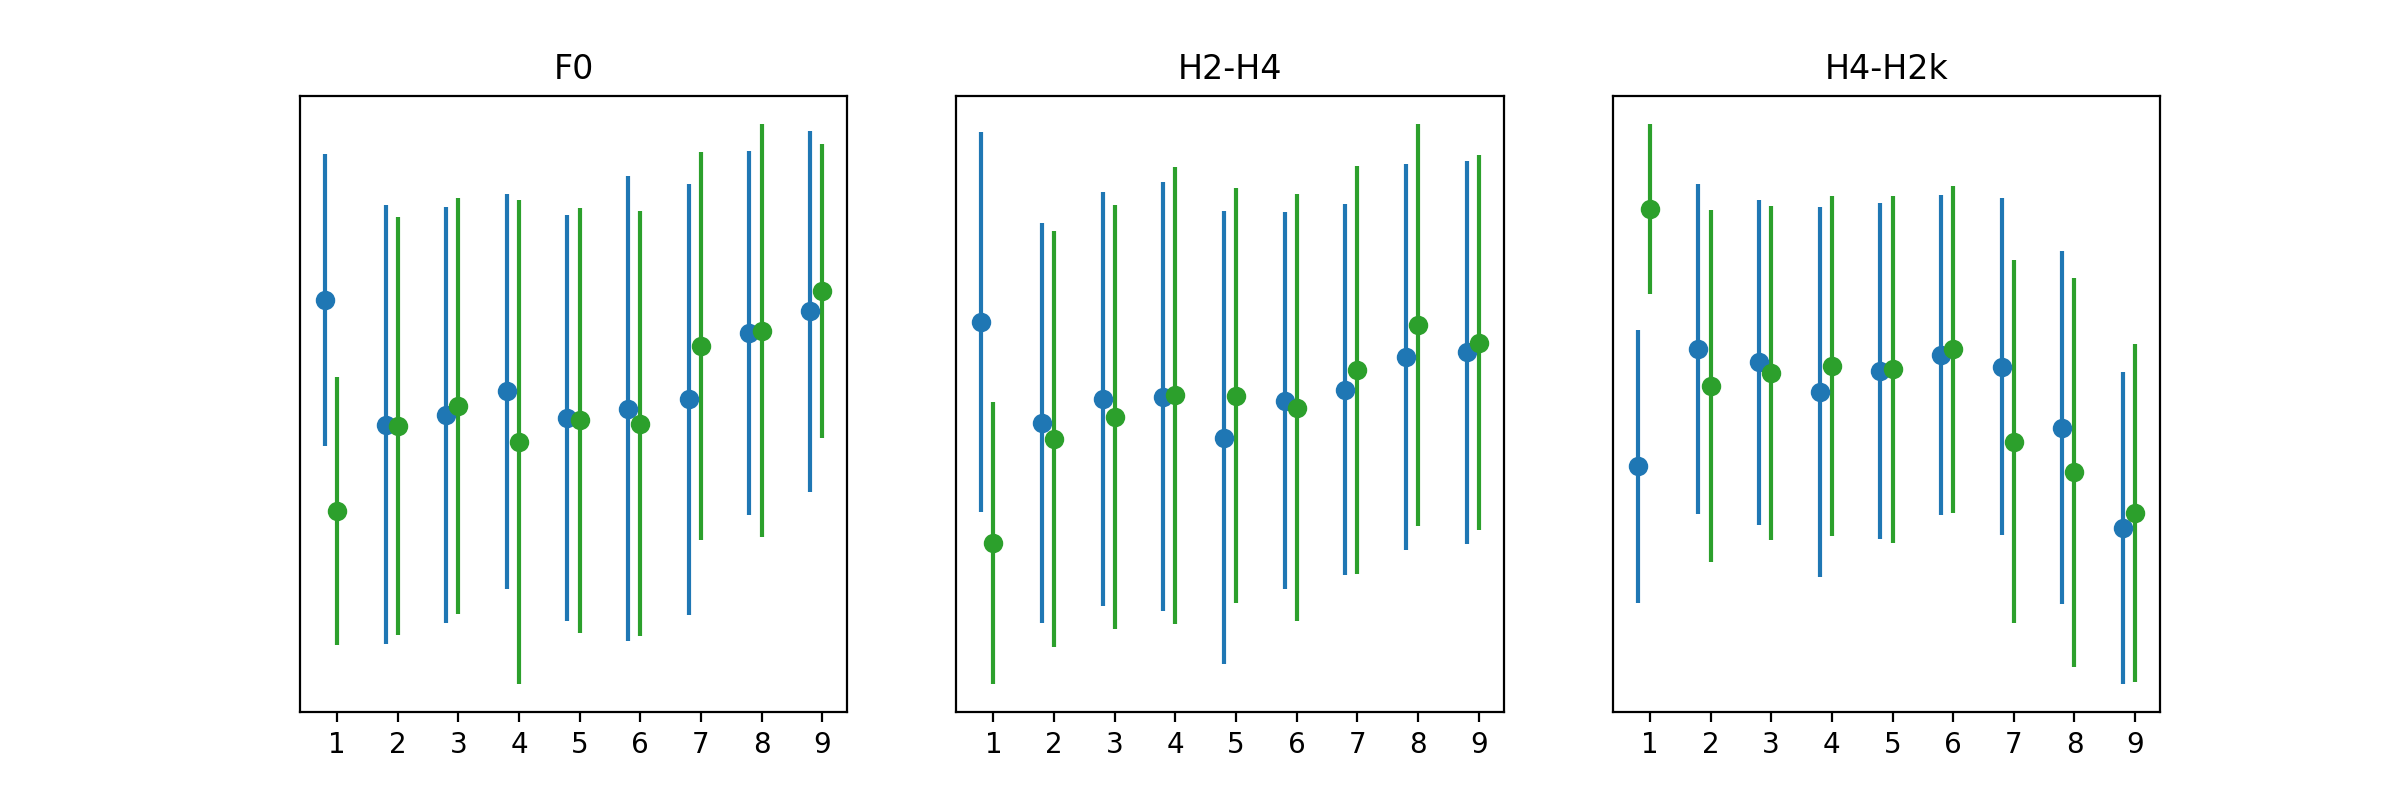
\includegraphics[width=\linewidth]{IS2019_paper_kit/images/errbar_VQual_clstr_flase.png}
%     \caption{\label{fig:vqual}Caption}
% \end{figure}


\subsection{Mel-Frequency Cepstral Coefficients}

Mel-frequency cepstral coefficients (MFCCs) are widely used acoustic features for classification \Amber{paralinguistic studies instead of classification}.  This feature set represents the overall spectral envelope of speech signals, and is closely related to the vocal tract shape. Physiological changes related to sleepiness might shape the vocal tract in a certain way that can be reflected in the spectral envelope. Thus, the distribution of MFCCs over an utterance might provide information about the sleepiness state \Amber{degree of sleepiness}of the speaker.

MFCCs were extracted with a window size of 25 ms, a window shift of 10 ms, a pre-emphasis filter with coefficient 0.97, and a sinusoidal lifter with coefficient 22. A filter bank with 23 filters was used and 13 coefficients were extracted. We also used the first and second derivatives of MFCCs. The voice box toolkit was used to extract MFCC features~\cite{brookes1997voicebox}.

\subsection{Entropy}

Entropy values between frames were calculated as described in~\cite{you2004entropy}. MFCCs were obtained from the speech signal using a Hamming window of length 25 ms and a frame shift of 2.5 ms. A 30 ms rectangular window was applied to MFCCs and using the features within the window, the signal's local entropy was computed as:

\begin{equation}
    H(v) = K \ln{\sqrt{2\pi}} + \ln{\Tr({\Sigma})},
\end{equation}
where, $H(v)$ is the entropy of the random variable $v$ of dimension $K$. $\Sigma$ is the $ K \times K $ covariance matrix of the probability distribution function of the random variable $v$.  



If an acoustic feature changes rapidly, the entropy of an acoustic feature between frames would be high. 
Therefore, we expected entropy can be used to represent instantaneous speech rate.
In order to verify this hypothesis, the correlation between the number of syllables per second, a conventional speech rate measure, and the mean entropy within an utterance was calculated.
Syllables per second was computed using a Praat script as described in \cite{DeJong2009}.

The computed speech rate was highly correlated with the mean entropy of the training data, as shown in Figure~\ref{fig:entropy_rate}. The linear regression between the mean the speech rate and mean entropy resulted in $R^2=0.50$ and $p<0.001$.  The corresponding Pearson's correlation coefficient was 0.71. This high correlation provides an evidence to the hypothesis that entropy can be used to represent speech rate.
The unexplained variance in the linear regression might be due to the difference in information reflected in each methods.
For example, the syllables per second measure only focuses on syllable nuclei,
while the entropy reflects between-frame change over all frames in an utterance.
%Another possibility is in unexpected inaccuracies in the entropy and/or speech rate calculation algorithms. 


%While speech rate in terms of the number of syllables per second or words per minute can be calculated at the utterance level, entropy can be calculated frame by frame. The distribution of instantaneous speech rate might provide more information about sleepiness of the speaker than the average speech rate over an utterance. %Experimental results verified this hypothesis. 

\begin{figure}
    \centering
    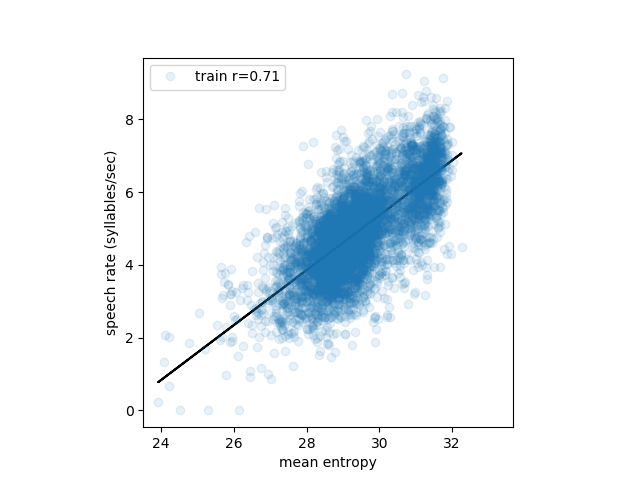
\includegraphics[width=\linewidth]{IS2019_paper_kit/images/scatter_train.png}
    \caption{\label{fig:entropy_rate}Scatter plot of speech rate in terms of syllables per second vs. mean of frame level change in entropy within an utterance in the training dataset. A line was fitted using the linear regression ($R^2=0.50$, $p<0.001$).}
\end{figure}

\subsection{ComParE16 Feature Set}

As the baseline acoustic feature set, the ComParE 2016 feature set was used \cite{weninger2013acoustics}. 
This set consists of $F_0$, energy, spectral, cepstral and voicing related frame-level features which are
referred to as low-level descriptors (LLDs). The set also includes the zero crossing rate, jitter, shimmer, harmonic-to-noise ratio (HNR), spectral harmonicity and psychoacoustic spectral
sharpness. In total, this feature set contains 6,373 static features resulting from the computation of various functionals over
low-level descriptor contours. These functionals are statistical,
polynomial regression coefficients and transformations on the
low-level descriptors. We used the TUMs open-source openSMILE system to extract the ComParE16 features~\cite{eyben2010opensmile} .